% Please make sure you insert your
% data according to the instructions in PoSauthmanual.pdf

%\documentclass[a4paper]{PoS}
%\documentclass{article}

\documentclass[prc,floatfix,superscriptaddress]{revtex4}

\usepackage{color}
\usepackage[normalem]{ulem}
\input epsf

\setlength{\textwidth}{6.5in}
\setlength{\textheight}{9.6in}
\setlength{\oddsidemargin}{0.0in}
\setlength{\topmargin}{-1.0in}
\usepackage{amsmath}
\usepackage{graphicx}
\usepackage{url}
\usepackage{color}
\usepackage{subfigure}
\usepackage{longtable}
\usepackage{dcolumn}



    % See p.105 of "TeX Unbound" for suggested values.
    % See pp. 199-200 of Lamport's "LaTeX" book for details.
    %   General parameters, for ALL pages:
    \renewcommand{\topfraction}{0.9}	% max fraction of floats at top
    \renewcommand{\bottomfraction}{0.8}	% max fraction of floats at bottom
    %   Parameters for TEXT pages (not float pages):
    \setcounter{topnumber}{2}
    \setcounter{bottomnumber}{2}
    \setcounter{totalnumber}{4}     % 2 may work better
    \setcounter{dbltopnumber}{2}    % for 2-column pages
    \renewcommand{\dbltopfraction}{0.9}	% fit big float above 2-col. text
    \renewcommand{\textfraction}{0.07}	% allow minimal text w. figs
    %   Parameters for FLOAT pages (not text pages):
    \renewcommand{\floatpagefraction}{0.7}	% require fuller float pages
	% N.B.: floatpagefraction MUST be less than topfraction !!
    \renewcommand{\dblfloatpagefraction}{0.7}	% require fuller float pages

	% remember to use [htp] or [htpb] for placement

\newcommand*{\JLAB}{Thomas Jefferson National Accelerator Facility, Newport News, Virginia 23606, USA}
\newcommand*{\WILL}{William I. Fine Theoretical Physics Institute, University of
Minnesota, Minneapolis, MN 55455, USA}
\newcommand*{\SCHOOL}{School of Physics and Astronomy, University of Minnesota, Minneapolis, MN 55455, USA}
\newcommand*{\ITEP}{Institute of Theoretical and Experimental Physics, Moscow, 117218, Russia}


\newcommand{\GPDtE}{\langle \tilde{E} \rangle}
\newcommand{\GPDtH}{\langle \tilde{H} \rangle}

\newcommand{\GPDHT}{\langle H_T \rangle}
\newcommand{\GPDETbar}{\langle \bar{E}_T \rangle}

\newcommand{\HT}{\langle H_T \rangle}
\newcommand{\ETbar}{\langle \bar{E}_T \rangle}





\begin{document}
\title{Cross Section Model for the $\pi^0$ and $\eta$ exclusive electroproduction processes}


\author {Valery Kubarovsky\\ \JLAB} 
\maketitle
\section{Introduction}	
The cross section of the exclusive   $\pi^0$ and $\eta$ electroproduction reaction $ep\to e^\prime p^\prime \pi^0/\eta$ was measured at Jefferson Lab  with a 5.75-GeV electron beam and the CLAS detector. Differential cross sections $d^4\sigma/dtdQ^2dx_Bd\phi$ and  structure functions $\sigma_U = \sigma_T+\epsilon\sigma_L, \sigma_{TT}$ and $\sigma_{LT}$, as functions of $t$ were obtained over a wide range of $Q^2$ and $x_B$.  
At low $t$, both  $\pi^0$ and $\eta$ are described reasonably well by Generalized Parton Distributions (GPDs)  in which chiral-odd transversity GPDs are dominant. 
Generalized form factors of the transversity GPDs $\HT^{\pi,\eta}$ and $\ETbar^{\pi,\eta}$ were directly extracted from the experimental observables
as a function of  $t, x_B$ and $Q^2$.  These form factors were parametrized by simple expressions with few parameters that were determined using CLAS6 data set. The program package includes functions for calculating  of the $ep\to\pi^0/\eta p$ cross section ,  structure functions 
$\sigma_T,\ \sigma_{TT}\ and\ \sigma_{LT}$ and generalized form factors $\HT$ and $\ETbar$. The MC generator for the reactions $ep\to\pi^0/\eta p$ was written based on these package.





%%%%%%%%%%%%%%%%%%%%%    SECTION   STRUCTURE FUNCTIONS %%%%%%%%%%%%%%%%%%%%%%%%%%%%%%%%%%%%%%%%%%%%%
\section{Definition of the structure functions}

The experimental four-fold differential cross section as a function of the four variables $(Q^2,x_B,t ,\phi_\eta)$ was obtained from the expression
(see \cite{clas1,clas2,clas3} for more details)
\begin{equation}
\begin{split}
\frac{d^4 \sigma_{ep \rightarrow e^\prime p^\prime (\pi^0/\eta)}}{dQ^2 dx_B dt d\phi_\eta} = 
 \frac{N(Q^2,x_B,t,\phi_\eta)}{\mathcal{L}_{int} (\Delta Q^2  \Delta x_B \Delta t \Delta \phi)} \times \\
\frac{1}{\epsilon_{ACC}\delta_{RC} \delta_{Norm}Br(\eta\to\gamma\gamma)}.
\end{split}
\label{eq:sig_ep_eppippim}
\end{equation}


The reduced or ``virtual photon"  cross sections  were extracted from the the four-fold differential cross section


\begin{equation}
\frac{d^2\sigma_{\gamma^* p \rightarrow p^\prime (\pi^0/\eta)} }{dt d\phi} = 
\frac{1}{\Gamma_V(Q^2,x_B,E)} 
\frac{d^4\sigma_{ep\rightarrow e^\prime p^\prime (\pi^0/\eta)}}{dQ^2 dx_B dt d\phi}.
\label{RXS}
\end{equation}

\noindent
The Hand convention  was adopted for the
definition of the virtual photon flux $\Gamma_V$: 

\begin{equation}
\Gamma_V (Q^2,x_B,E)= \frac{\alpha}{8\pi} \frac{Q^2}{m^2 E^2} 
\frac{1-x_B}{x_B^3} \frac{1}{1-\epsilon},
\label{eq:GammaV}
\end{equation}
\noindent where $\alpha$ is the standard electromagnetic coupling constant, $m$ is the nucleon mass and $E$ is the beam energy.
The variable $\epsilon$ represents the ratio of fluxes of longitudinally  and transversely polarized virtual photons and is given by
\begin{equation}
\epsilon=\frac {1-y-\frac{Q^2}{4E^2}}   {1-y+\frac{y^2}{2}+\frac{Q^2}{4E^2} }
\label{epsilon},
\end{equation}
with $y=p \cdot q/q \cdot k=\nu/E$.



The unpolarized reduced meson cross section is described 
 by 4 structure functions $\sigma_T$, $\sigma_L$, $\sigma_{TT}$ and $\sigma_{LT}$:
\begin{equation}
2\pi\frac{d^2\sigma(\gamma^*p\to p\pi^0)}{dtd\phi_\pi} = 
\frac{d\sigma_T}{dt} + 
\epsilon  \frac{d\sigma_L} {dt}+ 
\epsilon  \frac{d\sigma_{TT}} {dt}  \cos 2\phi+
\sqrt{2\epsilon (1+\epsilon)}   \frac{d\sigma_{LT}} {dt}  \cos \phi.
\label{Eq:Reduced}
\end{equation}
\noindent
$\phi$ is the angle between the lepton and hadron planes. The lepton plane
is defined by the incident and the scattered electron. The hadron plane
is defined by the meson and the scattered proton.

\noindent 
References~\cite{Goloskokov:2011rd,GL} obtain the following relations for unpolarized structure functions:

\begin{equation}
\label{SL}
\frac{d\sigma_{L} }{dt}= \frac{4\pi\alpha}{k}\frac{1}{Q^2}\left\{ \left( 1-\xi^2 \right) \left|\GPDtH\right|^2 -2\xi^2 {Re}\left[ \GPDtH^* \GPDtE \right] - \frac{t^\prime}{4m^2} \xi^2 \left| \GPDtE \right|^2 \right\}
\end{equation}

\begin{equation}
\label{ST}
\frac{d\sigma_{T}}{dt} = \frac{4\pi\alpha}{2k Q^4} \left[ \left(1-\xi^2\right) \left|\GPDHT\right|^2 - \frac{t'}{8m^2} \left|\GPDETbar\right|^2\right]
\end{equation}

\begin{equation}
\label{SLT}
\frac{d\sigma_{LT}}{dt} = \frac{4\pi\alpha}{\sqrt{2}k Q^3} \xi \sqrt{1-\xi^2} \frac{\sqrt{-t'}}{2m} { Re} \left[ \langle H_T\rangle^* \langle\tilde{E}\rangle \right]
\end{equation}

\begin{equation}
\label{STT}
\frac{d\sigma_{TT}}{dt} = \frac{4\pi\alpha}{k Q^4}\frac{t'}{16m^2}\left|\GPDETbar\right|^2
\end{equation}

\noindent 
Here  $t^\prime =t-t_{min}$, where $|t_{min}|$ is the minimum value of $|t|$ corresponding to $\theta_\pi =0$, $k(Q^2,x_B)$ is a phase space factor and  $\bar E_T = 2\widetilde H_T + E_T$.
The brackets $\langle  H_T \rangle$ and $\langle \bar E_T \rangle$ denote
the convolution of the elementary process 
$\gamma^*q\to q\pi^0$
with the GPDs $H_T$ and $\bar E_T$. We call them generalized form factors.

Phase space factor
\begin{equation}
\label{ps}
k=16\pi(W^2-m^2)\sqrt{\Lambda(W^2,-Q^2,m^2)},
\end{equation}
\noindent
where
\begin{equation}
\label{LAMBDA}
\Lambda(W^2,-Q^2,m^2)=W^4+Q^4+m^4+2W^2Q^2-2W^2m^2+2Q^2m^2.
\end{equation}
At high $Q^2$ the phase space factor behaves as $k\sim Q^4$. Taking this into account we conclude that 
$\sigma_L\sim Q^{-6}$,
$\sigma_T\sim Q^{-8}$,
$\sigma_L{TT}\sim Q{-^8}$ and 
$\sigma_{LT}\sim Q{^7}$ as expected.


%%%%%%%%%%%%%%%%%%%%%%%%%%%%%%%%%%%%%%%%%%%%%%%%%%%%%%%%%%%%%%%%%%%%%%%%%%%
\begin{figure*}[t!]
\centering
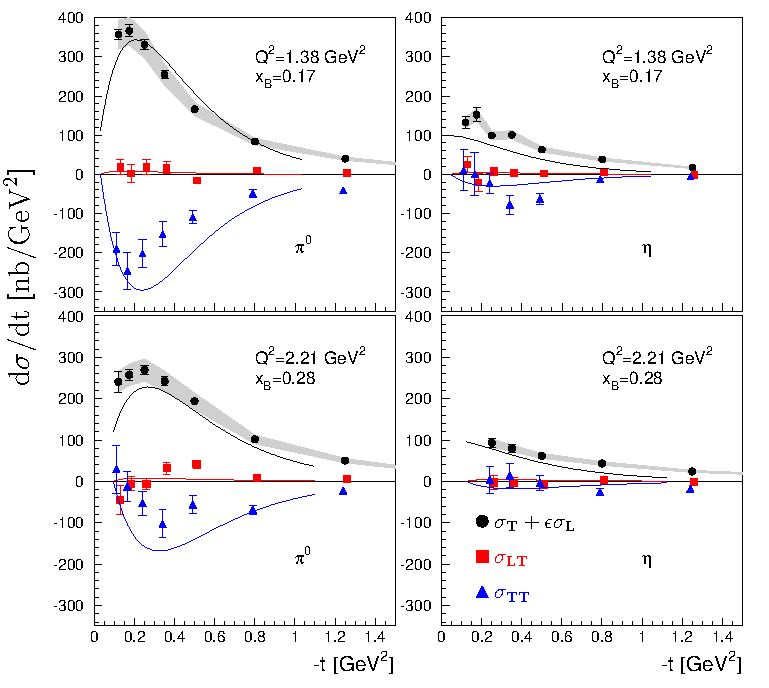
\includegraphics[height=8cm] {fig16_scissored.pdf}
\caption
{The extracted structure functions vs. $t$ for 
the $\pi^0$ (left column) 
%~\cite{Agashe:2014kda} 
and $\eta$ (right column). The top row presents data for the kinematic point  ($Q^2=$1.38~GeV$^2$,$x_B$=0.17)
and bottom row for the kinematic point ($Q^2=$2.21~GeV$^2$,$x_B$=0.28). 
The data and curves are as follows:  
black circles - $d\sigma_U/dt =d\sigma_T/dt +\epsilon d\sigma_L/dt$,
blue triangles - $d\sigma_{TT}/dt$,
red  squares - $d\sigma_{LT}/dt$.
The error bars are statistical only. The gray bands are our estimates of the absolute normalization systematic uncertainties on $d\sigma_U/dt $.
The curves are theoretical predictions produced  with the GPG model of Goloskokov and Kroll~\cite{Goloskokov:2011rd}.
}
\label{fig:structure}
\end{figure*} 



%%%%%%%%%%%%%%%%     PI0 and ETA data  %%%%%%%%%%%%%%%%%%%%%%%
\section{Experimental data}
Cross section of the reaction $ep\rightarrow ep(\pi^0/\eta)$ measured by 
the CLAS collaboration at Jlab in bins of $Q^2$, $x_B$, $t$ and $\phi$ were published in 
 Refs.
 \cite{clas1,clas2,clas3}.
Structure functions $\sigma_U=\sigma_T+\epsilon\sigma_L$, $\sigma_{LT}$ and $\sigma_{TT}$ have been obtained. These functions were compared 
with the predictions of the GPD models \cite{Goloskokov:2011rd,GL}. CLAS confirmed that the measured unseparated cross sections are much larger than expected from 
leading-twist handbag calculations which are dominated by longitudinal photons. 
The comparison of the $\pi^0$ and $\eta$ structure functions is shown in Fig.~\ref{fig:structure} for two kinematics as an example. 
$\sigma_U$ drops by a factor of 2.5 for $\eta$ in comparison with $\pi^0$ and
$\sigma_{TT}$ drops by a factor of 10.
However the GK GPD model \cite{Goloskokov:2011rd}  (curves)  follows the experimental data.
The inclusion of $\eta$ data into consideration strengthens 
the statement about the transversity GPD dominance in the pseudoscalar electroproduction process.
%################################ FIGURE ht_et_pi0 ##########################

\begin{figure}[t!]
\vspace*{-10 mm}
\centerline{
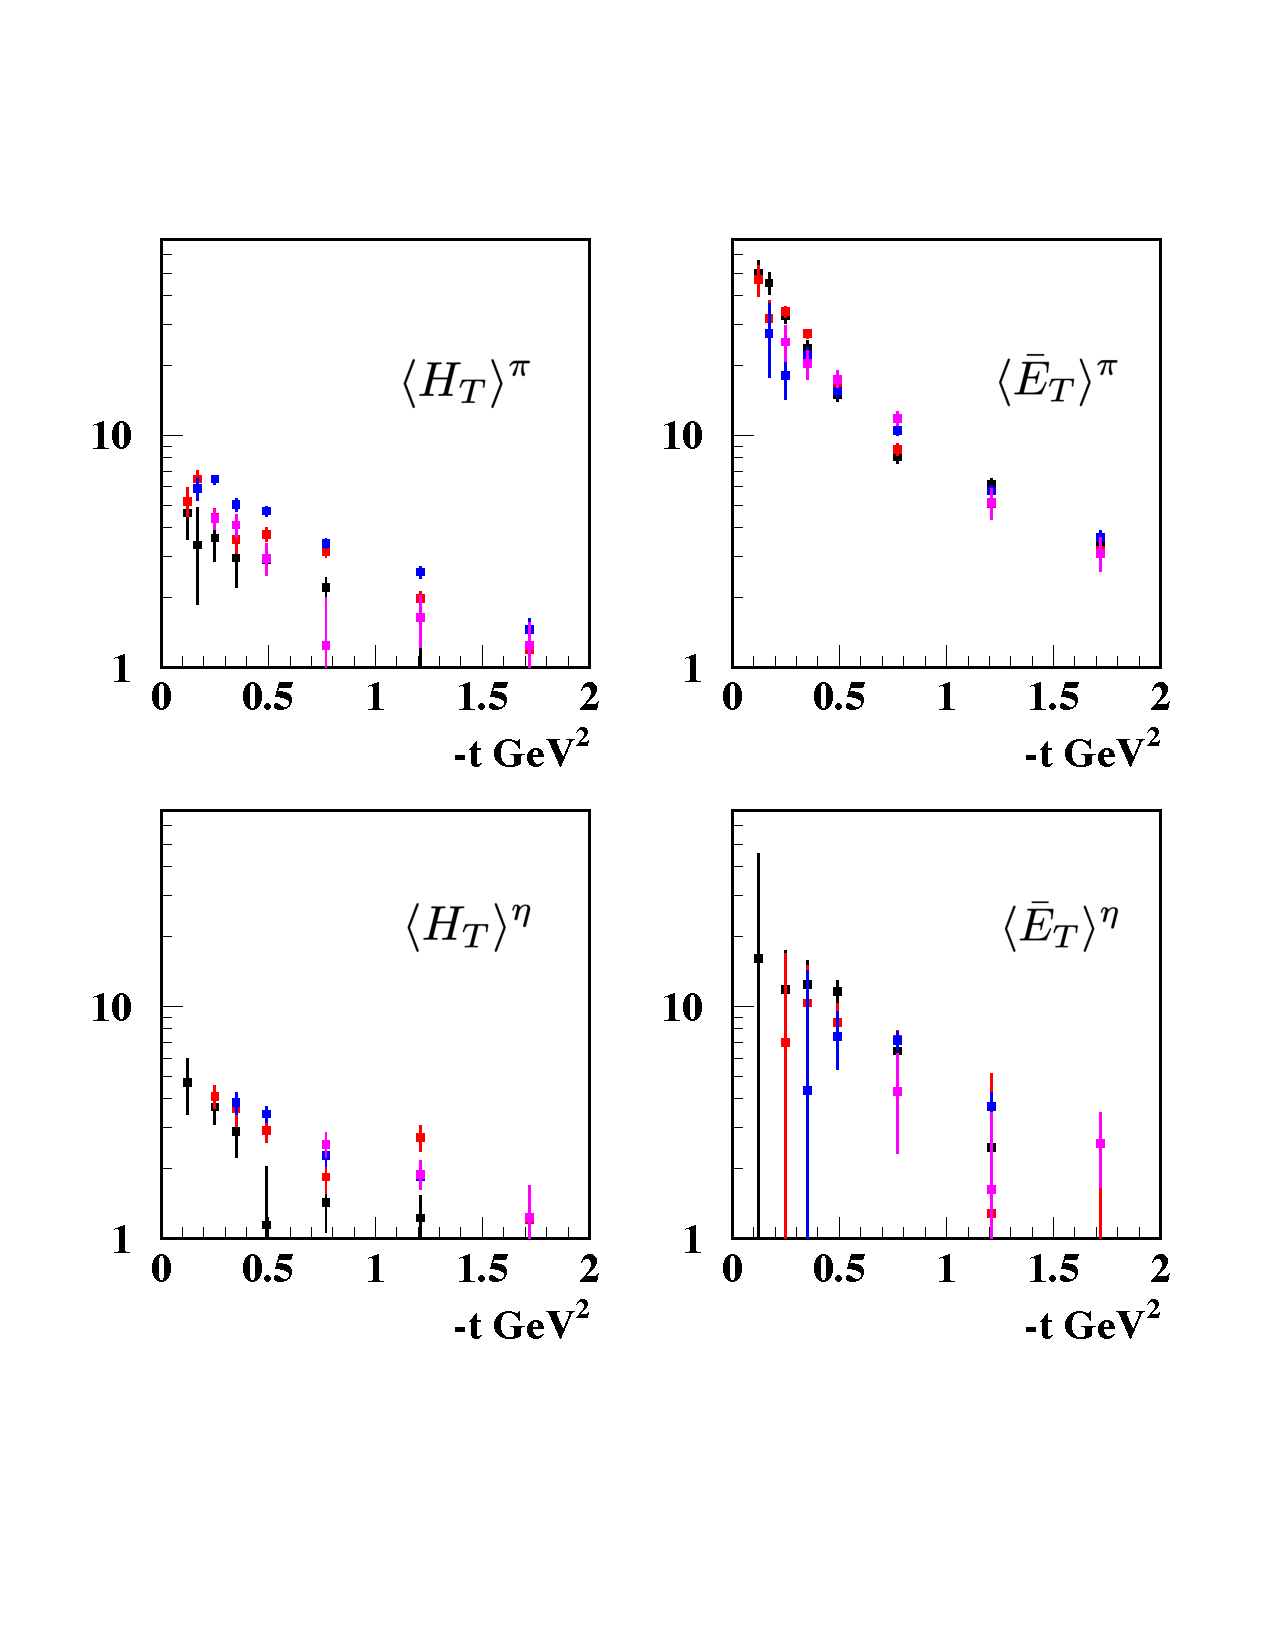
\includegraphics[height=15cm]{ht_et_pi0_eta.pdf}
}
\vspace*{-27mm}
\caption{ Data points: CLAS.
Top left: $\left|\GPDHT^\pi\right|$,
top right: $\left|\GPDETbar^\pi\right|$,
bottom left: $\left|\GPDHT^\eta\right|$,
bottom right: $\left|\GPDETbar^\eta\right|$ as a function of -$t$ for different kinematics:
($Q^2$=1.2 $GeV^2$,$x_B$=0.15) black, 
($Q^2$=1.8 GeV$^2$,$x_B$=0.22) red, 
($Q^2$=2.2 GeV$^2$,$x_B$=0.29) blue, 
($Q^2$=2.7 GeV$^2$,$x_B$=0.34) magenta. 
}
\label{fig:ht_et_pi0_eta}
\end{figure}


%%%%%%%%%%%%%%

\begin{figure}[h!]
\vspace*{-10 mm}
\centerline{
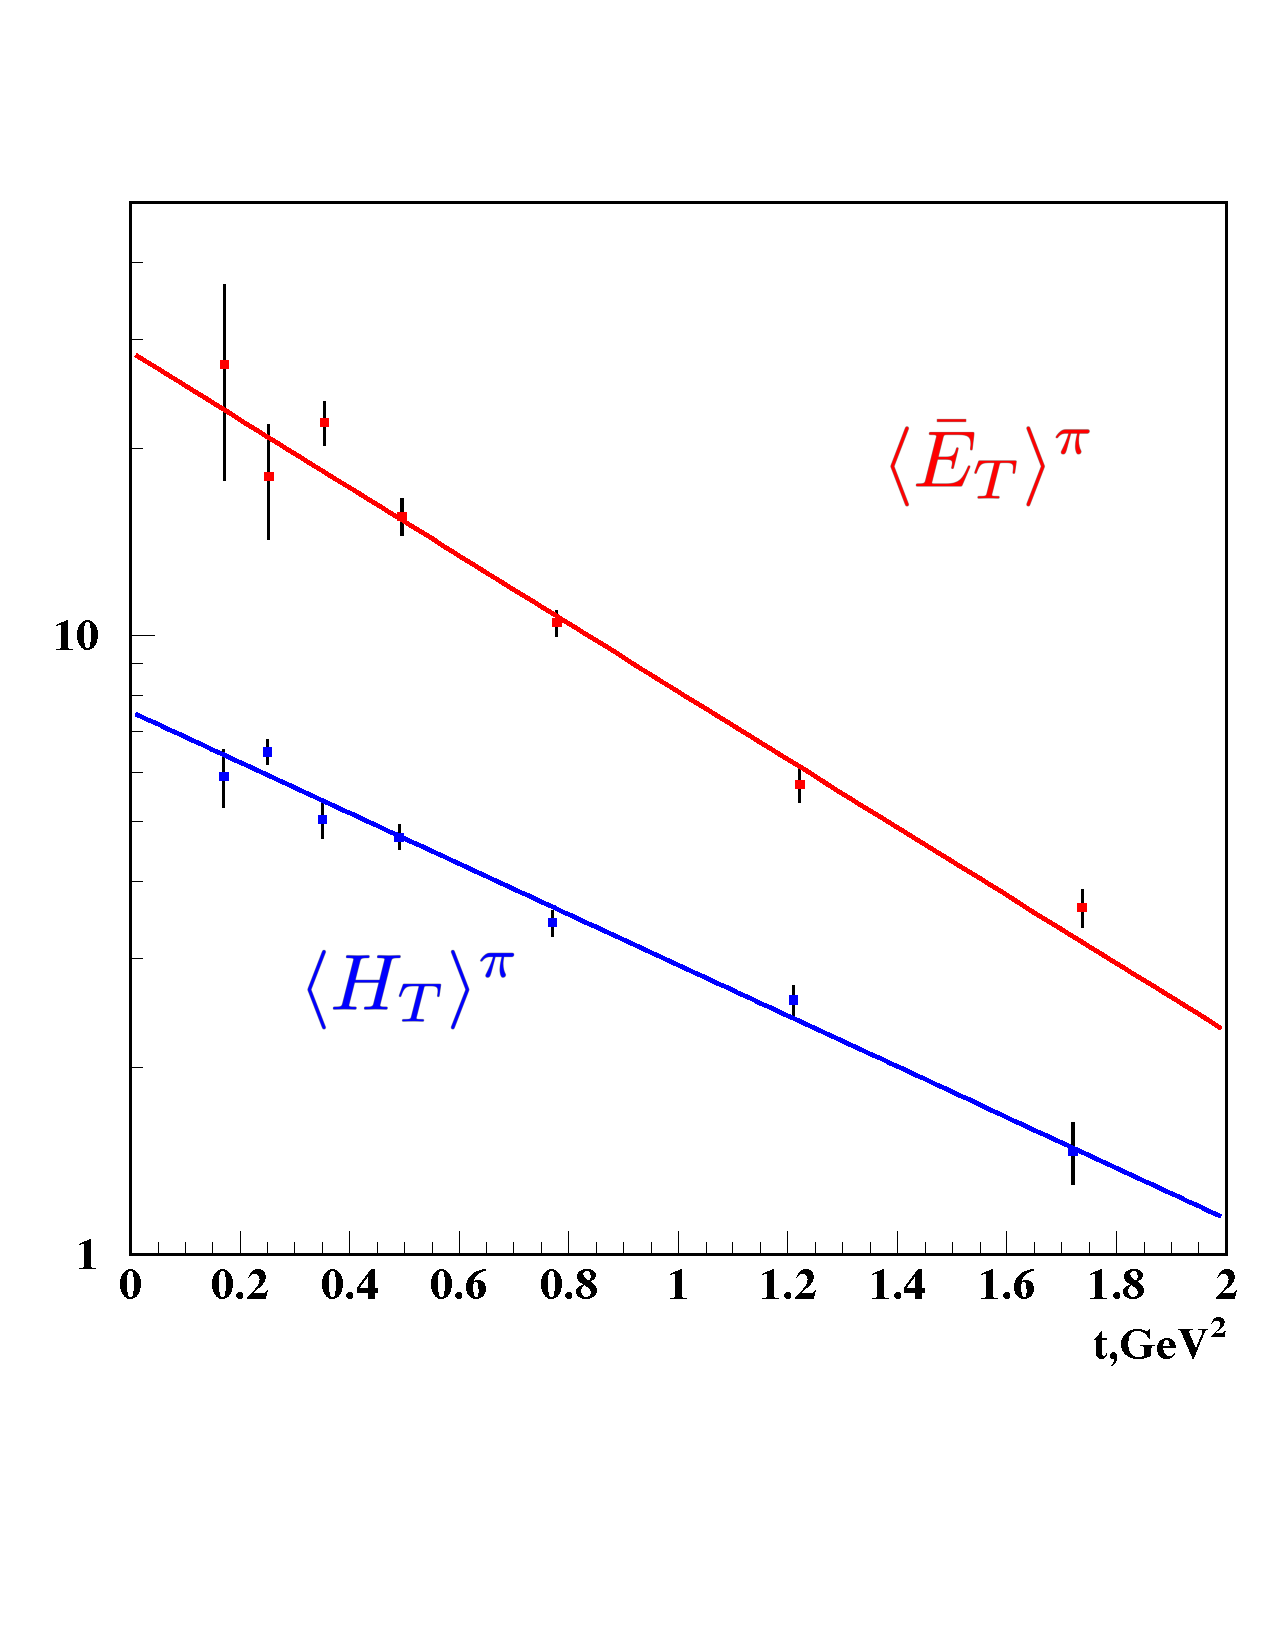
\includegraphics[width=8cm]{ht_et_pi.pdf}
}
\vspace*{-25 mm}
\caption
{
Generalized form factors $|\GPDHT^\pi|$   and $|\GPDETbar^\pi|$. 
Top: $|\GPDETbar^\pi|$ in red; 
Bottom: $|\GPDHT^\pi|$ in blue;
as a function of -$t$ for $Q^2=2.2~GeV^2$  and $x_B$=0.27.
}
\label{fig:ht_et_pi0}
\end{figure}


%%%%%%%%%%%%%%%%    GENERALIZED FORM FACTORS     %%%%%%%%%%%%%%%%%%

\section{Generalized form factors}
The squared magnitudes of the 
generalized form factors
$\left|\GPDHT\right|^2$ and 
$\left|\GPDETbar\right|^2$  
may be directly extracted from the experimental data (see Eqs. \ref{ST} and \ref{STT} ) in the framework of GPD models.
\begin{equation}\label{ET}
\left|\GPDETbar^{\pi,\eta}\right |^2=\frac{k^\prime Q^4}{4\pi\alpha}     \frac{16m^2}{t'} \frac{d\sigma^{\pi,\eta}_{TT}}{dt} 
\end{equation}
\begin{equation}\label{HT}
\left| \GPDHT^{\pi,\eta}\right|^2=\frac{2k^\prime Q^4}{4\pi\alpha}       \frac{1}{1-\xi^2} \left [ \frac{d\sigma^{\pi,\eta}_{T}}{dt} + \frac{d\sigma^{\pi,\eta}_{TT}}{dt} \right ].
\end{equation}
\noindent
Fig.~\ref{fig:ht_et_pi0_eta} presents the modules of the generalized form factors
$\left|\GPDHT^\pi\right|$, $\left|\GPDETbar^\pi\right|$, $\left|\GPDHT^\eta\right|$ and $\left|\GPDETbar^\eta\right|$
 for 4 different kinematics. 
  Note the dominance of the $\left|\GPDETbar\right|$ over $\left|\GPDHT\right|$ for both $\pi^0$ and $\eta$.
Generalized form factors $\GPDHT^\pi$ and $\GPDETbar^\pi$ are shown for one kinematics at Fig.~\ref{fig:ht_et_pi0} in more details. 
 $\GPDETbar^\pi$ has steeper t-dependemce than $\GPDHT^\pi$. The t-slope parameters from the fit by  
 exponential function $e^{bt}$ are 
 $b(\GPDETbar)$=1.27~$GeV^{-2}$ and $b(\GPDHT)$=0.98~$GeV^{-2}$.
 The $t$-dependence can be described by the exponential function $e^{bt}$. The slope paremeter $b$ is a function of $x_B$ and $Q^2$.

%%%%%%%%%%%%%%%%%%%%%%   PARAMETRIZATION  %%%%%%%%%%%%%%%%%%%%%%%

\section{Parametrization of the Generalized form factors}
There are 8 parameters used in the model  for the $\GPDHT$   and $\GPDETbar$ Generalized form factors in the model:  

\begin{equation}
\label{GFF:HT}
\GPDHT(t,x_B,Q^2)=p_1\cdot \exp[p_2+p_3(\ln x_B-\ln0.15)t]\cdot Q^{p_4}
\end{equation}

\begin{equation}
\label{GFF:ET}
\GPDETbar(t,x_B,Q^2)=p_6\cdot \exp[p_7+p_8(\ln x_B-\ln0.15)t]\cdot Q^{p_9}
\end{equation}

It turned out that the $x_B$-dependence of the generalized form factors $\HT$ and $\ETbar$ is very week. By this reason we drop $x_B$-dependence
in the form factors parametrization.
\begin{itemize}
\item $p_{1,6}$ -- normalization factor
\item $p_{2,7}$ --  determines the t-slope parameter: $e^{p_{2,7}t}$
\item $p_{3,8}$ -- determines the t-slope parameter, correlated with  $x_B$ $e^{(p_{3,8}\ln{x_B} )t}$
\item $p_{4,9}$ -- determines the $Q^2$ -dependence
\end{itemize}
It was shown in the CLAS publications \cite{clas2,clas3} that the t-slope parameters depends on the $x_B$ variable. This behavior also follows from the GPD models.
The term $\ln0.15$ added for the convenience. The parameter $p_2$ equals to the slope parameter exactly at $x_B=0.15$ with such a definition of the parameter's set.

Due to the lack of statistics we are using only 2 parameters for the parametrization of the $\sigma_{LT}$ structure function
\begin{equation}
\label{GFF:RE}
\sqrt{Re[\GPDHT^*\GPDtE]}=p_{11}\cdot \exp(p_{12}t)
\end{equation}
Structure function $\sigma_L=0$ in our model.

 We have 10 parameters in total in this model.  We used published CLAS6 data \cite{clas2,clas3} of the  reduce cross sections 
$\gamma^*p\to (\pi^0/\eta) p$ 
(Eq. \ref{Eq:Reduced})  to fit the data and to determine the model parameters.
The cross section (Eq. \ref{Eq:Reduced}) and structure functions (Eq. \ref{SL}, \ref{ST}, \ref{SLT}, \ref{STT}) are the functions of the generalized form-factors Eq. \ref{GFF:HT}, \ref{GFF:ET}, \ref{GFF:RE}. The fit parameters of these generalized form-factor are presented in 
Table \ref{Tab:pi0_fit_parameters} for $\pi^0$-electroproduction and in 
Table \ref{Tab:eta_fit_parameters} for $\eta$-electroproduction.

The comparison of the model and experimental data are presented in Fig. \ref{fig:pi0_sf},\ref{fig:eta_sf},\ref{fig:pi0_gff} and \ref{fig:eta_gff}.

\section{Description of the program functions}

The package includes the calculation of the cross sections and structure functions  for two sets of the variables:
\begin{enumerate}
\item $x_b,Q^2,t,\phi$
\item $\cos\theta,W,Q^2,\phi$
\end{enumerate}




\begin{enumerate} 
\item     REAL FUNCTION DVMPX(del2,xB,Q2, Phi\_g,E,heli,MESONMASS)

This function returns the differential cross section 
$$
\frac{d^4 \sigma}{dQ^2 dx_B dt d\phi} [{ep \rightarrow e^\prime p^\prime (\pi^0/\eta)}]\ \ \ \ \ \mu b/Gev^4
$$
         \begin {itemize}
                  \item del2 is the  momentum transfer $t$, negative ($GeV^2$)
                  \item $\phi$ is the  angle in the photon frame (radians)
                  \item $xB$ is the Bjorken variable $x_B$
                  \item $Q2$ is  $Q^2$ ($GeV^2$)
                  \item $E$  is the  beam energy (GeV)
                  \item $heli$ is the  beam helicity
                  \item $ MESONMASS$ is the mass of the meson ($m_\pi$ or $m_\eta$) (GeV)
         \end{itemize}
The structure function can be calculated separately:
\begin{itemize}
\item         REAL FUNCTION XSIGMA\_L(del2,xB,Q2,E)

This function returns the structure function $\frac{d\sigma_L}{dt}(t,x_b,Q^2,E)=0$
\item         REAL FUNCTION XSIGMA\_U(del2,xB,Q2,E)

This function returns the structure function $\frac{d\sigma_T}{dt}(t,x_b,Q^2,E)$
\item         REAL FUNCTION XSIGMA\_TT(del2,xB,Q2,E)

This function returns the structure function $\frac{d\sigma_{TT}}{dt}(t,x_b,Q^2,E)$
\item         REAL FUNCTION XSIGMA\_LT(del2,xB,Q2,E)

This function returns the structure function $\frac{d\sigma_{LT}}{dt}(t,x_b,Q^2,E)$
\end{itemize}


 \item Subroutine DVMPW(COST,W,Q2, Phi\_g,E,heli,MESONMASS, S\_T, S\_L, S\_TT, S\_LT, S\_LTP)
        \begin {itemize}
                  \item COST=$\cos(\theta)$, where $\theta$ is the  angle in the CM system (pi0-gamma* or  p-p') of the reaction $\gamma^*+p\to Meson+p$ 
                  \item W is W (GeV)
                  \item Phi\_g is the  angle in the photon frame (radians)
                  \item $xB$ is the Bjorken variable $x_B$
                  \item $Q2$ is  $Q^2$ ($GeV^2$)
                  \item $E$  is the  beam energy (GeV)
                  \item $heli$ is the  beam helicity
                  \item $ MESONMASS$ is the mass of the meson ($m_\pi$ or $m_\eta$) (GeV)
         \end{itemize}

	This subroutine calculates the structure functions
	\begin{itemize}
		\item S\_T=$\frac{d\sigma_T}{d\cos\theta}(\cos\theta,W,Q^2,E)$
		\item S\_L=$\frac{d\sigma_L}{d\cos\theta}(\cos\theta,W,Q^2,E)$
		\item S\_TT=$\frac{d\sigma_{TT}}{d\cos\theta}(\cos\theta,W,Q^2,E)$
		\item S\_LT=$\frac{d\sigma_{LT}}{d\cos\theta}(\cos\theta,W,Q^2,E)$
		\item S\_LTP=$\frac{d\sigma_{LTP}}{d\cos\theta}(\cos\theta,W,Q^2,E)$
	\end{itemize}

\end{enumerate}




%%%%%%%%%%%%%%%%%%%%%%%%  TABLES %%%%%%%%%%%%%%%%%%%%%%%%%%%%%%%%%%%%%

\begin{table}[h!]
\caption{Fit parameters for $\pi^0$ electroproduction}
\begin{tabular}{   | c | c | c |  c | c |}
\hline
                  &  $\GPDHT$                  & $ \ETbar$ &  $\sqrt{Re[\GPDHT^*\GPDtE]}$    \\
\hline
$p_{1,6}$  & \ 6.262 $\pm$ 0.130  & 92.972  $\pm$ 2.466 &    \\
$p_{2,7}$  &\  0.803  $\pm$ 0.009& \ 3.407  $\pm$ 0.020&    \\
$p_{3,8}$   & -0.115  $\pm$ 0.016& \  -1.909 $\pm$ 0.023&    \\
$p_{4,9}$  & \  1.743 $\pm$ 0.058 &\  -0.119  $\pm$  0.099 &  \\
\hline
$p_{11}$  &   &   &   16.860  $\pm$1.406 \\
$p_{12}$  &   &   & \ \   2.172  $\pm$0.168 \\
\hline
\end{tabular}
\label{Tab:pi0_fit_parameters}
\end{table}

%%%%%%%%%%%%%%%%%%%%%%%%%%%%%%%%%%%%%%%%%%%%%%%%%%%%%%%%%%%%%
\begin{table}[h!]
\caption{Fit parameters for $\eta$ electroproduction}
\begin{tabular}{   | c | c | c |  c | c |}
\hline
                  &  $\GPDHT$                  & $ \ETbar$ &  $\sqrt{Re[\GPDHT^*\GPDtE]}$    \\
\hline
$p_{1,6}$  & \ 6.943 $\pm$ 0.261  & 17.042  $\pm$ 1.416 &    \\
$p_{2,7}$  &\  1.752  $\pm$ 0.023& \ 1.126  $\pm$ 0.028&    \\
$p_{3,8}$   & -1.287  $\pm$ 0.022& \  0.049 $\pm$ 0.066&    \\
$p_{4,9}$  & \  0.682 $\pm$ 0.126 &\  1.659  $\pm$  0.311 &  \\
\hline
$p_{11}$  &   &   &   21.637  $\pm$5.283 \\
$p_{12}$  &   &   & \ \   3.987  $\pm$0.818 \\
\hline
\end{tabular}
\label{Tab:eta_fit_parameters}
\end{table}

\section{GITHUB Repository}

The code can be downloaded from the githup repository:

\href{https://github.com/vkubarovsky/Model-for-the-pi0-eta-exclusive-cross-section}{$\pi^0/\eta$ cross section model}.

The package consists of 4 subdirectories:
\begin{enumerate}
\item Functions

There are 3 functions in this directory.
\begin{enumerate}
\item dvmpx.F(t,xB,Q2,phi,Ebeam,Helicity, Mesonmass)
\item dvmw.F(CosTheta,W,Q2,$\phi$,Ebeam, helicity,Mesonmass,$\sigma_{T}$, $\sigma_{L}$, $\sigma_{TT}$, $\sigma_{LT}$, $\sigma_{LTP}$)
\item Exclurad.F

The package to calculate the radiative corrections for the reaction $ep\to e'p'(pi^0/\eta$.
\end{enumerate}
\item Test\_plots

The PAW kumac plot\_sf.kumac produces all plots
\item Tex

pi\_eta\_model.pdf  is the description of the package.
\item Pi0\_eta\_fit\_GFF

PAW code to fit the model parameters. The main kumac file is fit\_xs.kumac
\end{enumerate}






The $\pi^0/\eta$ generator based on this model is located in the githup repository

\href{https://github.com/drewkenjo/aao_norad}{$\pi^0/\eta$ generator}.




%%%%%%%%%%%%%%

\begin{figure}[t!]
\vspace*{-10 mm}
\centerline{
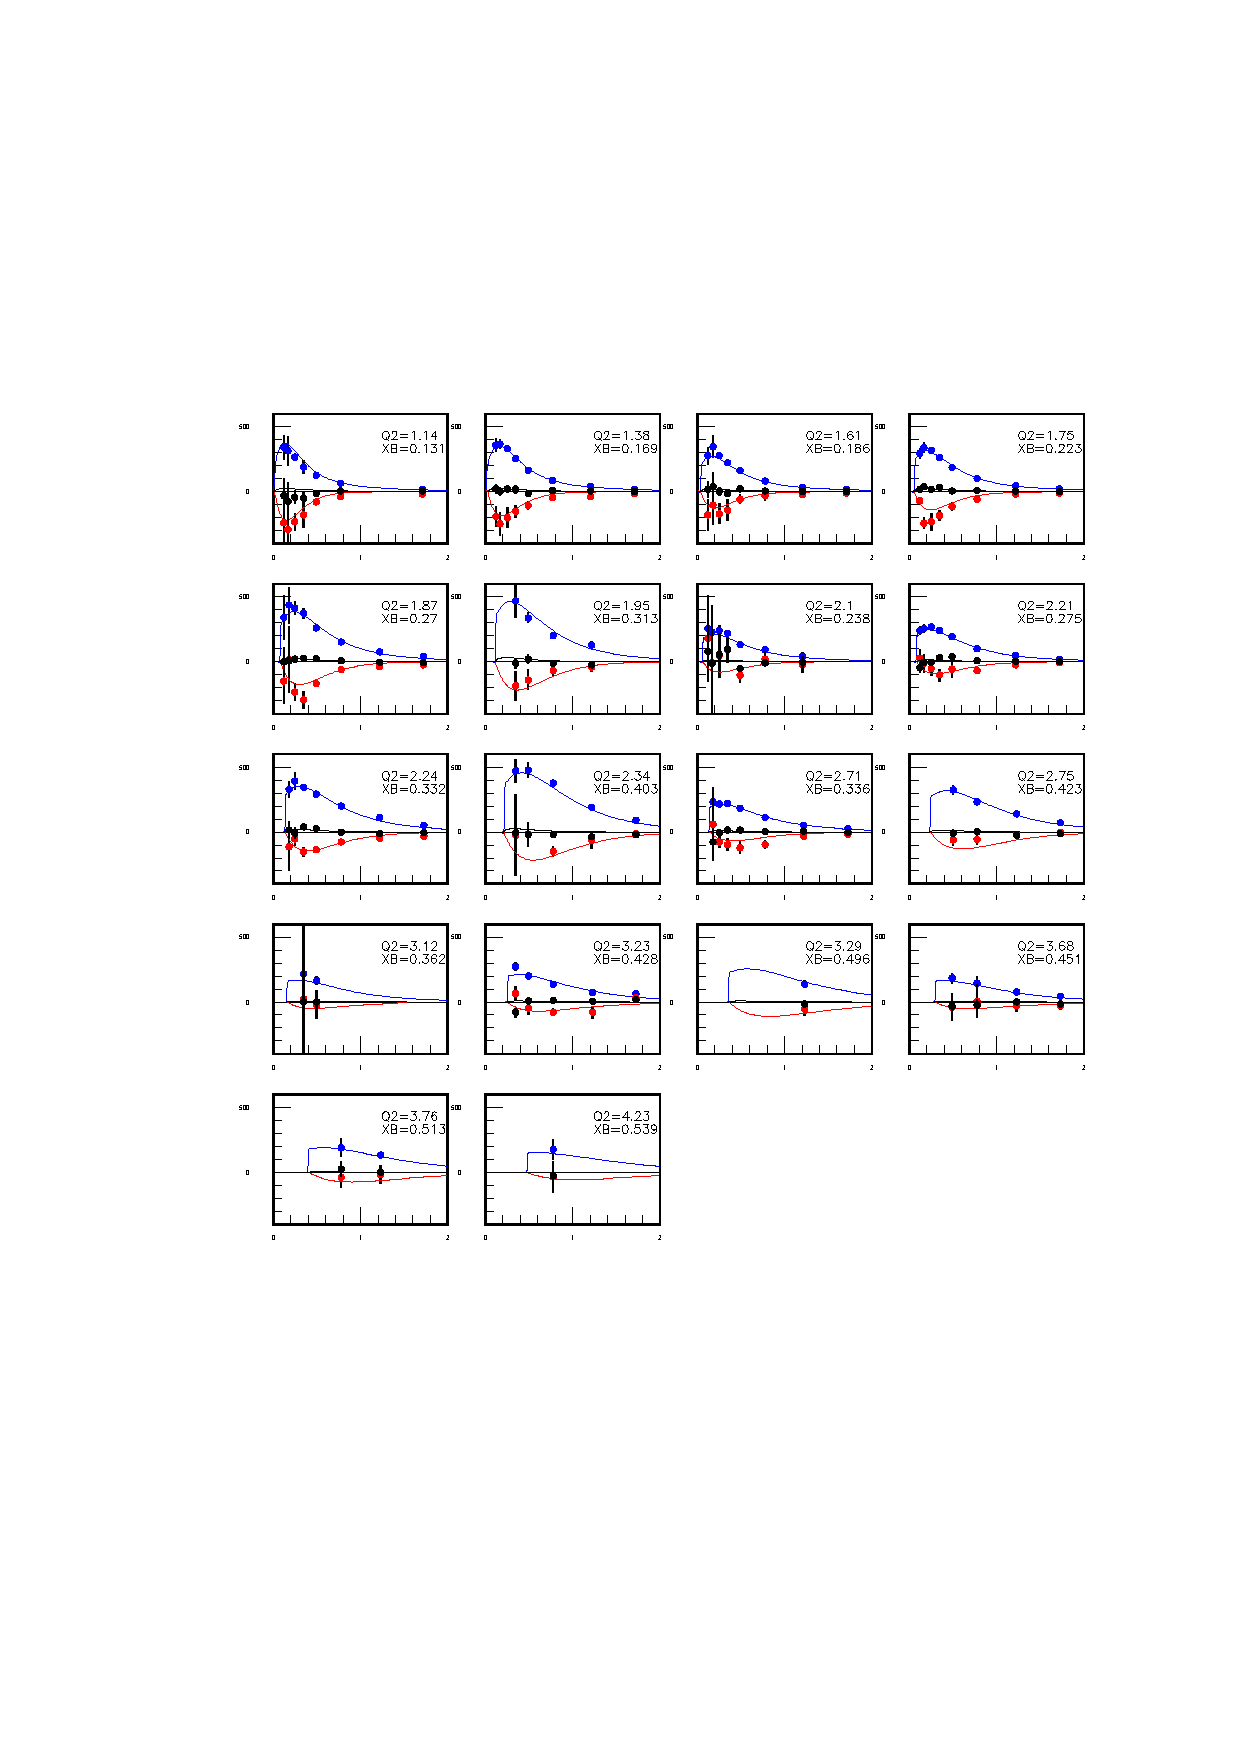
\includegraphics[height=30cm]{../Test_plots/pi0_sf.pdf}
\label{pi0_sf}
}
\vspace*{-70mm}
\caption{Comparison of CLAS6 data with the model for the $\pi^0$ electroproduction:
Blue: $\sigma_T$;
Red: $\sigma_{TT}$;
Black: $\sigma_{LT}$ as a function of $-t$.
}
\label{fig:pi0_sf}
\end{figure}

%%%%%%%%%%%%%%

\begin{figure}[t!]
\vspace*{-10 mm}
\centerline{
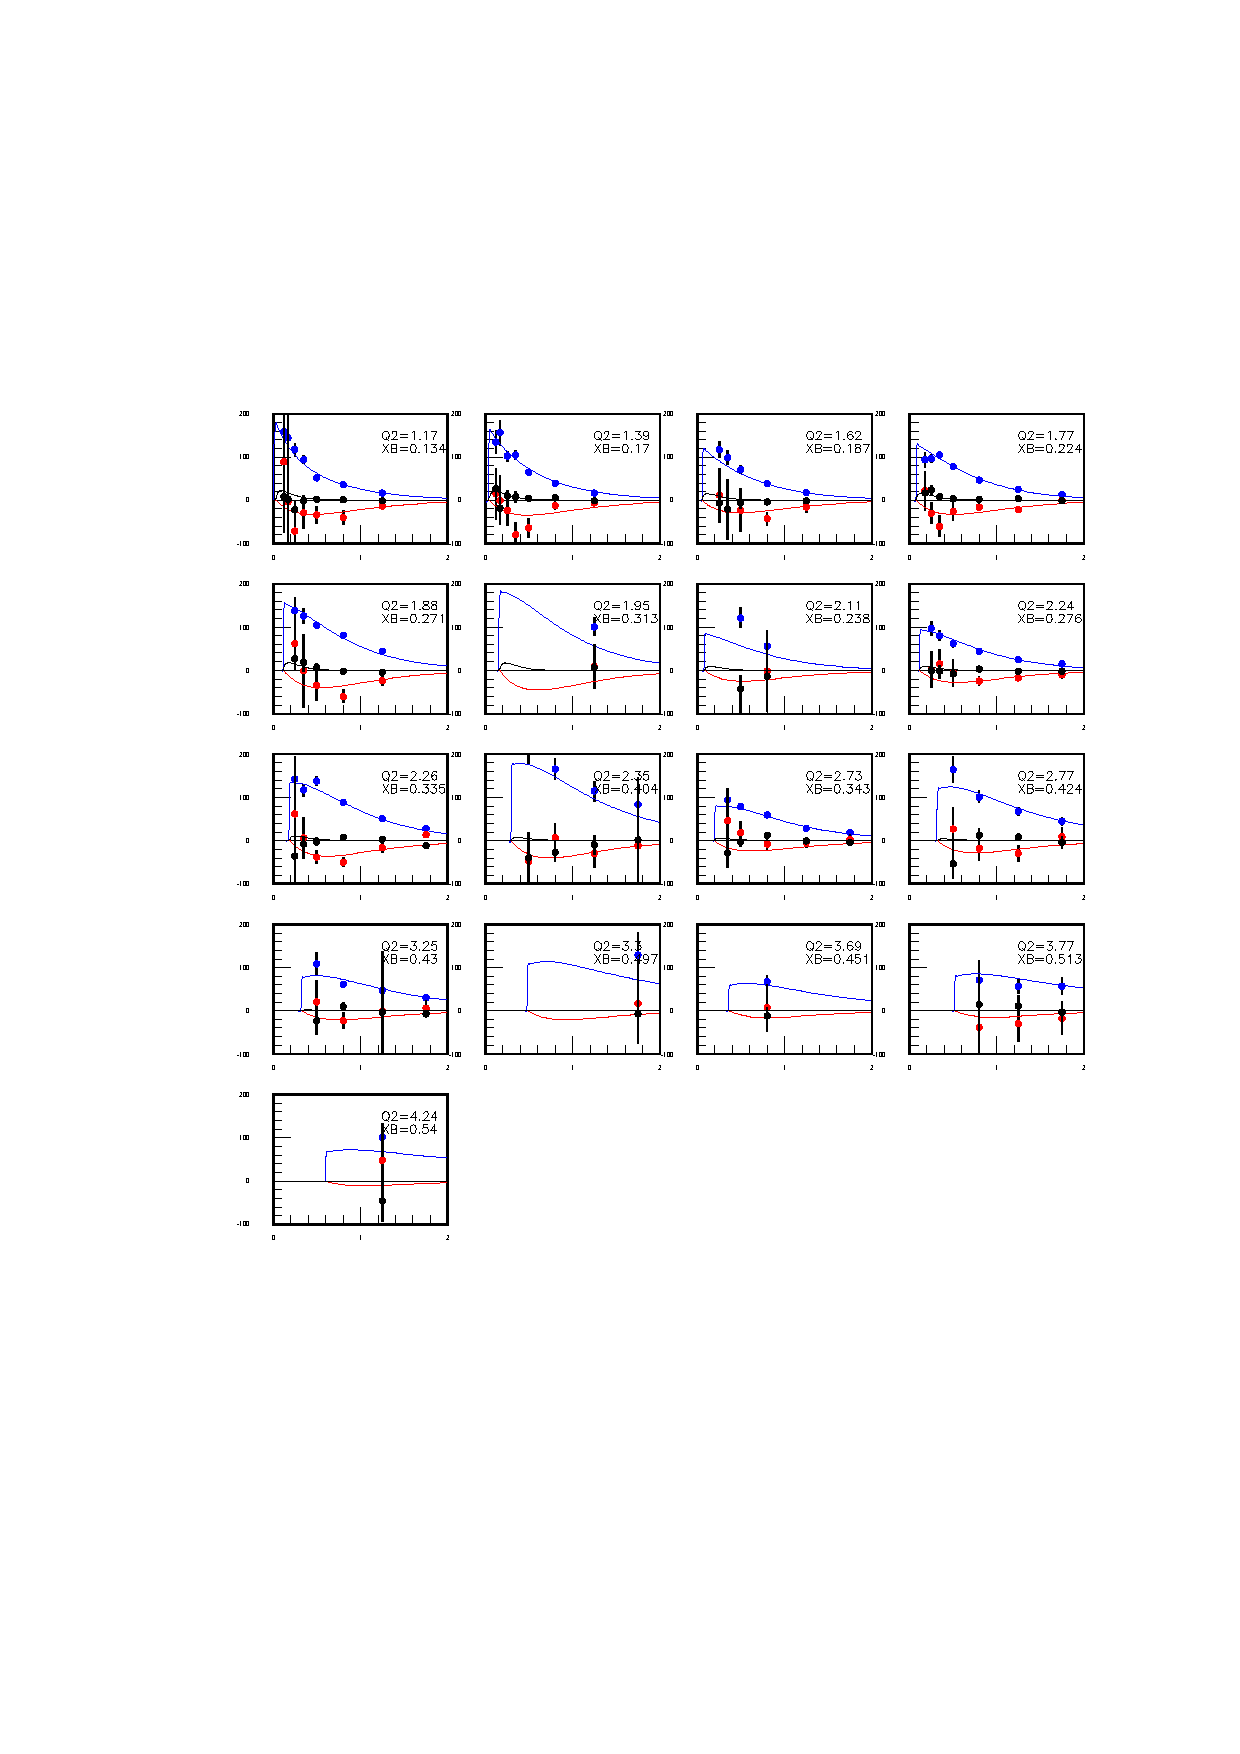
\includegraphics[height=30cm]{../Test_plots/eta_sf.pdf}
}
\label{eta_sf}
\vspace*{-70mm}
\caption{Comparison of CLAS6 data with the model for the $\eta$ electroproduction:
Blue: $\sigma_T$;
Red: $\sigma_{TT}$;
Black: $\sigma_{LT}$ as a function of $-t$.
}
\label{fig:eta_sf}
\end{figure}

%%%%%%%%%%%%%%%%%

\begin{figure}[t!]
\vspace*{-10 mm}
\centerline{

\includegraphics[height=30cm]{../Test_plots/pi0_HT2_ET2.pdf}
}
\label{pi0_gff}
\vspace*{-70mm}
\caption{Comparison of CLAS6 data with the model for the $\pi^0$ electroproduction:
Blue: $\GPDETbar$;
Red: $\GPDHT$,  as a function of $-t$.
}
\label{fig:pi0_gff}
\end{figure}

%%%%%%%%%%%%%%%%%%

\begin{figure}[t!]
\vspace*{-10 mm}
\centerline{
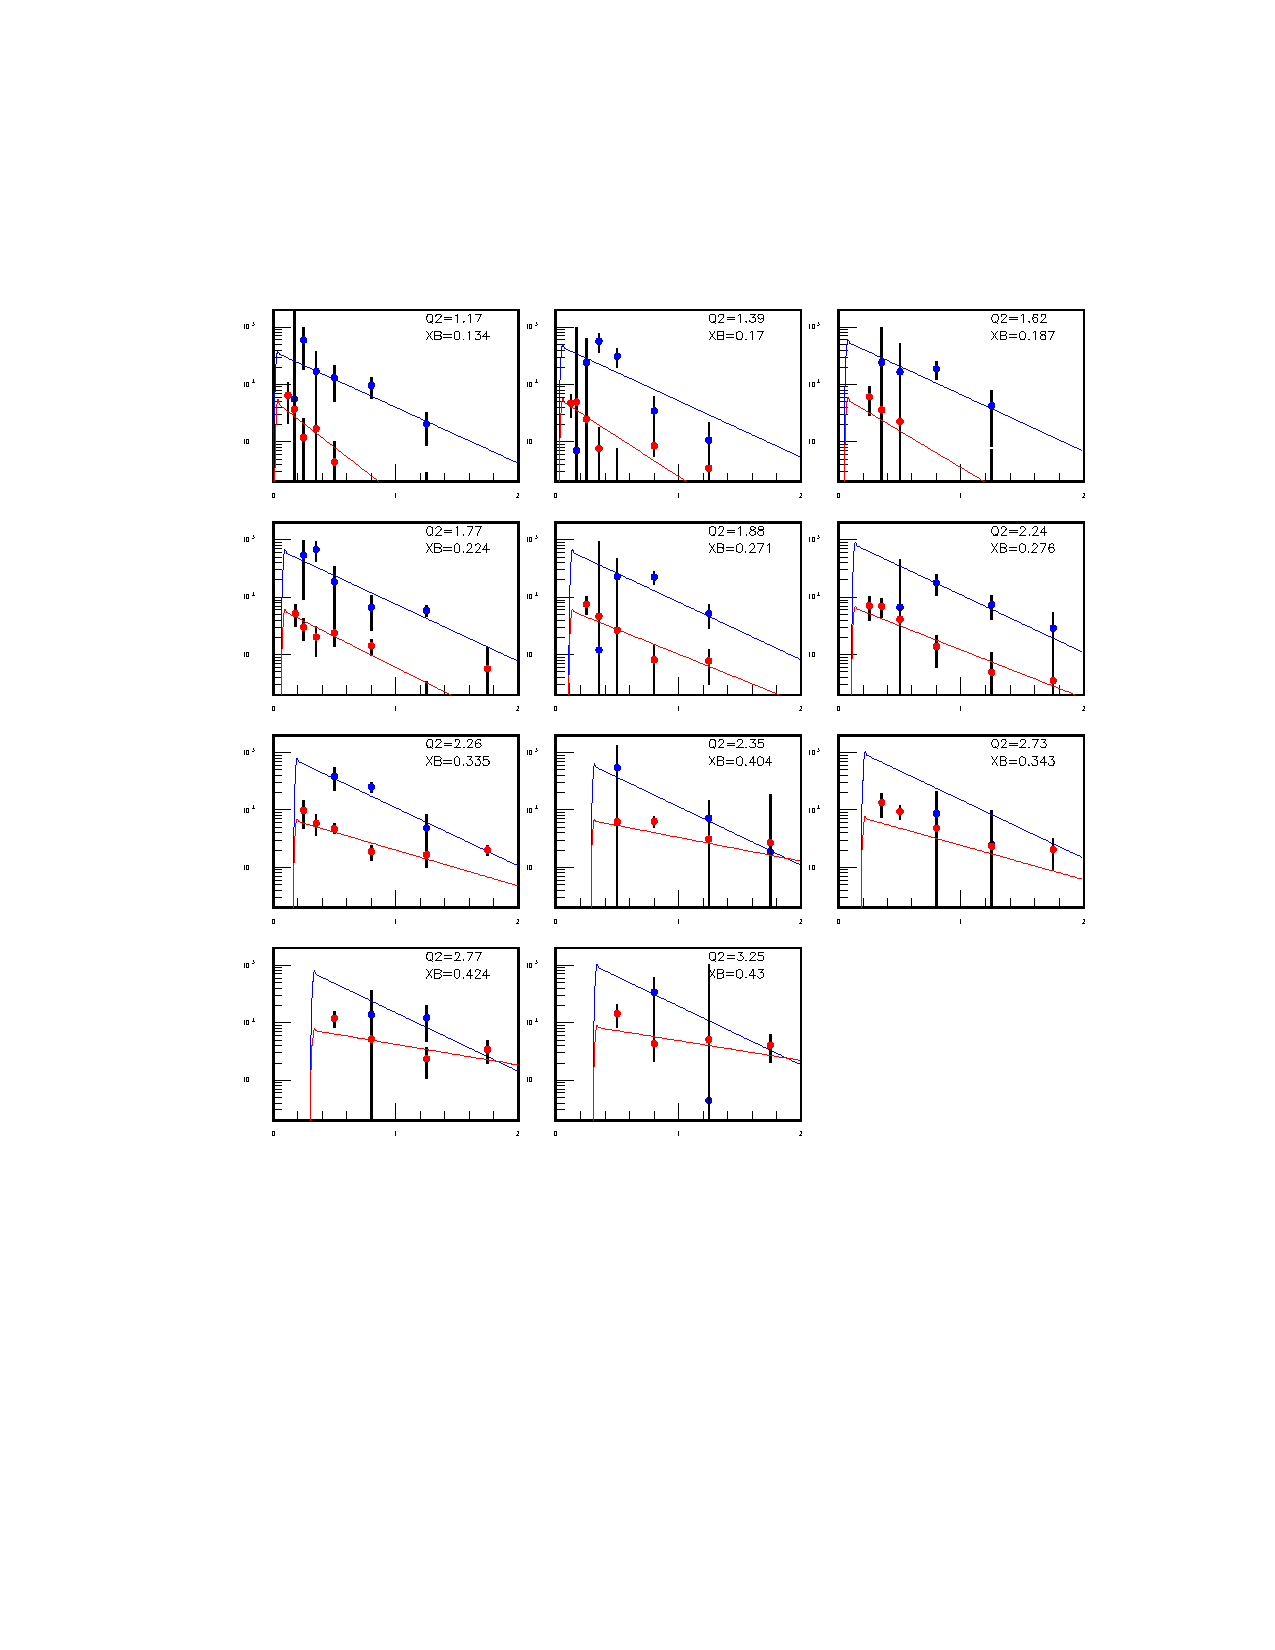
\includegraphics[height=30cm]{../Test_plots/eta_HT2_ET2.pdf}
}
\label{eta_gff}
\vspace*{-70mm}
\caption{Comparison of CLAS6 data with the model for the $\eta$ electroproduction:
Blue: $\GPDETbar$;
Red: $\GPDHT$  as a function of $-t$.
}\label{fig:eta_gff}
\end{figure}


%%%%%%%%%%%%%%    BIBLIOGRAPHY  %%%%%%%%%%%%%%%%%%%%%%%%%%%%%%%%%%%%

\begin{thebibliography} {0}

\bibitem{clas1} I. Bedlinskiy {\it et al.} (CLAS Collaboration), \emph{ Phys. Rev. Lett. }{\bf 109}, 112001 (2012). 
\bibitem{clas2} I. Bedlinskiy {\it et al.} (CLAS Collaboration), \emph{ Phys. Rev. C} {\bf 90}, 025205 (2014).
\bibitem{clas3} I. Bedlinskiy {\it et al.} (CLAS Collaboration), \emph{ Phys. Rev. C} {\bf 95}, 035202 (2017).

%\bibitem{Ji} X. Ji, \emph{ Phys. Rev. Lett.} {\bf78}, 610 (1997); \emph{ Phys. Rev. D} {\bf 55}, 7114 (1997).

%\bibitem{Radyushkin} A.V. Radyushkin, \emph{ Phys. Lett. B} {\bf380}, 417 (1996); \emph{ Phys. Rev. D} {\bf 56}, 5524 (1997).

%\bibitem{ji} P. Hoodbhoy and X.  Ji, \emph{ Phys. Rev.  D} {\bf58}, 054006 (1998).

\bibitem{Goloskokov:2011rd} S. V. Goloskokov and P. Kroll, \emph{ Eur. Phys. J. A} {\bf47}, 112 (2011).

\bibitem{GL}  G. Goldstein, J. O. Gonzalez-Hernandez  and S.~Liuti,%\bibitem{diehl} M. Diehl, \emph{ Phys. Rep.} {\bf 388}, 41 (2003) and references within.
\emph{ Phys. Rev. D }{\bf84}, 034007 (2011);
\emph{ Int. J. Mod. Phys. Conf. Ser. }{\bf20}, 222 (2012);
\emph{ J. Phys. G: Nucl. Part. Phys.} {\bf39} 115001 (2012).


%\bibitem{Ahmad:2008hp} S. Ahmad, G. R. Goldstein and S. Liuti, \emph{ Phys. Rev. D} {\bf79}, 054014 (2009).

%\bibitem{G-K-09} S. V. Goloskokov and P. Kroll, \emph{ Eur. Phys. J. C} {\bf65}, 137 (2010).



%\bibitem{Diehl:2005jf} M. Diehl and Ph. Hagler, Eur. Phys. J. C{\bf44}, 87 (2005)
%\bibitem{Gockeler:2006zu} M. Gockeler \emph{ et al.},  Phys. Rev. Lett. {\bf98}, 222001 (2007)



\end{thebibliography}

\end{document}

